\documentclass[UTF8,11pt,a4paper,oneside,fontset=none]{ctexart}

\usepackage[a4paper,top=1.72cm,bottom=1.72cm,left=1.82cm,right=1.82cm,headheight=15pt]{geometry}
\usepackage{fontspec}
\usepackage{amsmath,amssymb,mathtools,bm}
\usepackage{unicode-math}
\usepackage{booktabs,tabularx,array}
\usepackage[table]{xcolor}
\usepackage{enumitem}
\usepackage{fancyhdr}
\usepackage{caption}
\usepackage{hyperref}
\usepackage[most]{tcolorbox}
\usepackage{tikz}
\usetikzlibrary{arrows.meta,positioning}

\setmainfont{Times New Roman}
\setsansfont{Arial}
\setmonofont{Consolas}
\setmathfont{Cambria Math}
\setCJKmainfont[BoldFont=SimHei,ItalicFont=KaiTi]{SimSun}
\setCJKsansfont[BoldFont={Microsoft YaHei Bold}]{Microsoft YaHei}
\setCJKmonofont{FangSong}

\definecolor{DeepBlue}{HTML}{17324D}
\definecolor{PandaTeal}{HTML}{0B7A75}
\definecolor{WarmGold}{HTML}{C58A19}
\definecolor{Coral}{HTML}{C95F4A}
\definecolor{SoftBlue}{HTML}{EEF5F8}
\definecolor{SoftTeal}{HTML}{ECF7F5}
\definecolor{SoftGold}{HTML}{FFF7E7}
\definecolor{SoftRed}{HTML}{FFF0F0}
\definecolor{SoftGray}{HTML}{F5F7F9}
\definecolor{MidGray}{HTML}{667085}
\definecolor{LineGray}{HTML}{D5DEE5}

\hypersetup{
  colorlinks=true,
  linkcolor=DeepBlue,
  urlcolor=PandaTeal,
  pdfauthor={范子恒},
  pdftitle={PandaX-4T run10972 数据处理方法报告}
}

\ctexset{
  section={
    format=\Large\bfseries\color{DeepBlue},
    number=\arabic{section},
    beforeskip=0pt,
    afterskip=0.68em
  },
  subsection={format=\large\bfseries\color{PandaTeal}}
}

\pagestyle{fancy}
\fancyhf{}
\fancyhead[L]{\small\color{DeepBlue}PandaX-4T run10972}
\fancyhead[R]{\small\color{MidGray}数据处理方法报告}
\fancyfoot[C]{\small\color{MidGray}\thepage}
\renewcommand{\headrulewidth}{0.4pt}
\renewcommand{\footrulewidth}{0pt}

\captionsetup{font=small,labelfont=bf,labelsep=quad}
\setlength{\parindent}{2em}
\setlength{\parskip}{0.15em}
\setlist[itemize]{leftmargin=1.55em,itemsep=0.20em,topsep=0.22em,parsep=0pt}
\setlist[enumerate]{leftmargin=1.8em,itemsep=0.22em,topsep=0.22em,parsep=0pt}
\renewcommand{\arraystretch}{1.16}

\newcolumntype{Y}{>{\raggedright\arraybackslash}X}
\newcolumntype{C}[1]{>{\centering\arraybackslash}p{#1}}
\newcolumntype{R}[1]{>{\raggedleft\arraybackslash}p{#1}}

\newtcolorbox{infobox}[1][]{
  enhanced,breakable,colback=SoftBlue,colframe=DeepBlue,
  boxrule=0.7pt,arc=1.7mm,left=1.5mm,right=1.5mm,top=1.0mm,bottom=1.0mm,#1
}
\newtcolorbox{methodbox}[1][]{
  enhanced,breakable,colback=SoftTeal,colframe=PandaTeal,
  boxrule=0.75pt,arc=1.7mm,left=1.5mm,right=1.5mm,top=1.0mm,bottom=1.0mm,#1
}
\newtcolorbox{warningbox}[1][]{
  enhanced,breakable,colback=SoftGold,colframe=WarmGold,
  boxrule=0.75pt,arc=1.7mm,left=1.5mm,right=1.5mm,top=1.0mm,bottom=1.0mm,#1
}
\newtcolorbox{boundarybox}[1][]{
  enhanced,breakable,colback=SoftRed,colframe=Coral,
  boxrule=0.75pt,arc=1.7mm,left=1.5mm,right=1.5mm,top=1.0mm,bottom=1.0mm,#1
}
\newtcolorbox{codebox}[1][]{
  enhanced,breakable,colback=SoftGray,colframe=LineGray,
  boxrule=0.6pt,arc=1.2mm,left=2mm,right=2mm,top=1.0mm,bottom=1.0mm,
  fontupper=\small\ttfamily,#1
}

\newcommand{\SoneLY}{\mathrm{S1}}
\newcommand{\StwoLY}{\mathrm{S2B}}
\newcommand{\Rsixtyeight}{R_{68}}
\newcommand{\Rninty}{R_{90}}
\newcommand{\OOF}{\mathrm{OOF}}

\begin{document}

% -----------------------------------------------------------------------------
% 第 1 页：封面
% -----------------------------------------------------------------------------
\thispagestyle{empty}
\vspace*{0.85cm}
\noindent{\color{PandaTeal}\rule{\textwidth}{3.5pt}}

\vspace{0.95cm}
{\sffamily\bfseries\fontsize{25pt}{32pt}\selectfont\color{DeepBlue}
PandaX-4T run10972\par
数据处理方法报告\par}

\vspace{0.30cm}
{\sffamily\bfseries\fontsize{15.5pt}{21pt}\selectfont\color{PandaTeal}
事件级样本外重建、候选选择与不确定度评估\par}

\vspace{0.82cm}
\begin{tcolorbox}[
  colback=SoftBlue,colframe=DeepBlue,boxrule=0.9pt,arc=2mm,
  left=3mm,right=3mm,top=2.5mm,bottom=2.5mm
]
\centering
{\sffamily\bfseries\large 本报告回答的问题}\par
\vspace{1mm}
输入表怎样变成固定、可对齐的事件集合？\par
模型和权重怎样只在训练侧学习？\par
每个事件怎样得到一条真正未参与自身训练的 OOF 相对能量？
\end{tcolorbox}

\vspace{0.68cm}
\begin{center}
\begin{tabular}{C{4.65cm} C{4.65cm} C{4.65cm}}
\begin{tcolorbox}[width=4.4cm,colback=white,colframe=LineGray,arc=1.5mm,halign=center]
{\sffamily\bfseries\fontsize{22pt}{24pt}\selectfont\color{DeepBlue}4500}\par
\small 事件全部保留
\end{tcolorbox}
&
\begin{tcolorbox}[width=4.4cm,colback=white,colframe=LineGray,arc=1.5mm,halign=center]
{\sffamily\bfseries\fontsize{22pt}{24pt}\selectfont\color{PandaTeal}5}\par
\small 物理观测量
\end{tcolorbox}
&
\begin{tcolorbox}[width=4.4cm,colback=white,colframe=LineGray,arc=1.5mm,halign=center]
{\sffamily\bfseries\fontsize{22pt}{24pt}\selectfont\color{WarmGold}5\times900}\par
\small 平衡事件折
\end{tcolorbox}
\end{tabular}
\end{center}

\vspace{0.4cm}
\begin{boundarybox}[title={报告边界},fonttitle=\bfseries]
本文只说明数据处理方法，不重复原始数据分布，也不提前引用结果报告中的改善数值。当前输出是无量纲相对能量；没有单线真值和探测器增益时，不能把它直接标为 MeV。
\end{boundarybox}

\vfill
\begin{tabularx}{\textwidth}{@{}Y R{5.4cm}@{}}
\textbf{报告人：}范子恒 & \textbf{更新日期：}2026 年 7 月 18 日\\
\textbf{数据：}run10972 & \textbf{实现：}Python + LaTeX
\end{tabularx}

\vspace{0.32cm}
\noindent{\color{PandaTeal}\rule{\textwidth}{1.3pt}}
\clearpage

% -----------------------------------------------------------------------------
% 第 2 页：输入、对齐与流程
% -----------------------------------------------------------------------------
\section{输入、字段与唯一对齐键}

当前输入是一张上游生成的事件级标量表，而不是未经处理的探测器波形。程序始终只读原表，并把结果写入独立输出目录。主处理链只读取下面 7 个字段：
\begin{equation}
  \left\{
  \texttt{runNumber},\ \texttt{eventNumber},
  \texttt{qS1\_max},\ \texttt{qS2B\_max},
  \texttt{xS2T\_max},\ \texttt{yS2T\_max},\ \texttt{dt}
  \right\}.
\end{equation}
其中真正进入响应学习和能量组合的 5 个物理观测量是
\begin{equation}
  \symbf{x}_{i}
  =\bigl(\SoneLY_{i},\StwoLY_{i},x_i,y_i,t_{{\rm d},i}\bigr).
\end{equation}
\texttt{runNumber} 与 \texttt{eventNumber} 只用于描述来源，不作为响应特征，也不决定训练或测试归属。

\subsection*{1.1 用原始行序建立 \texttt{sourceRow}}

\texttt{eventNumber} 在表中可能重复，因此不能单独承担一一对齐。读入后、任何排序或处理之前，按照原始行序生成
\begin{equation}
  \texttt{sourceRow}_i=i,
  \qquad i=0,1,\ldots,4499.
\end{equation}
\texttt{sourceRow} 是本项目内部的唯一事件键。它不参与模型拟合，只用于对齐折标签、OOF 预测和原表行。输入内容或行序一旦改变，必须视为另一数据版本并重新生成全部结果。

\begin{center}
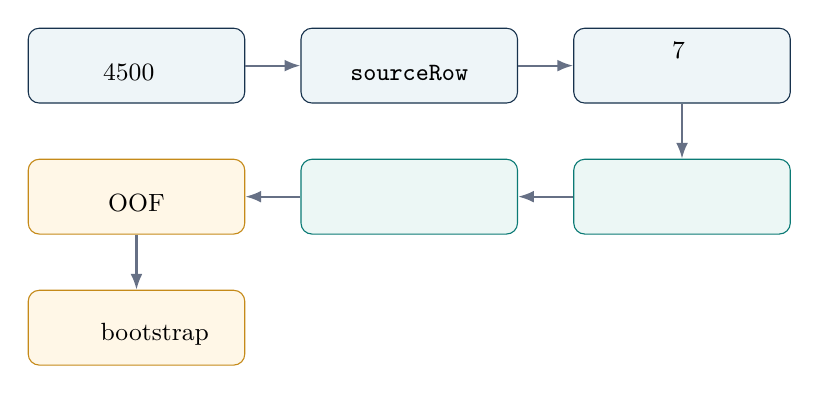
\begin{tikzpicture}[
  node distance=6mm and 7mm,
  every node/.style={font=\small,align=center},
  box/.style={draw=DeepBlue,fill=SoftBlue,rounded corners=1.4mm,minimum width=2.75cm,minimum height=0.95cm},
  teal/.style={draw=PandaTeal,fill=SoftTeal,rounded corners=1.4mm,minimum width=2.75cm,minimum height=0.95cm},
  gold/.style={draw=WarmGold,fill=SoftGold,rounded corners=1.4mm,minimum width=2.75cm,minimum height=0.95cm},
  arrow/.style={-{Latex[length=2mm]},thick,color=MidGray}
]
\node[box] (input) {只读标量表\\4500 行};
\node[box,right=of input] (key) {按原始行序生成\\\texttt{sourceRow}};
\node[box,right=of key] (audit) {检查 7 个字段\\有限值与正信号};
\node[teal,below=7mm of audit] (fold) {确定性随机\\事件级五折};
\node[teal,left=of fold] (learn) {训练侧拟合响应\\选择权重和方法};
\node[gold,left=of learn] (oof) {测试侧只应用\\保存 OOF 预测};
\node[gold,below=7mm of oof] (eval) {宽度、尾部与\\配对事件 bootstrap};
\draw[arrow] (input)--(key);
\draw[arrow] (key)--(audit);
\draw[arrow] (audit)--(fold);
\draw[arrow] (fold)--(learn);
\draw[arrow] (learn)--(oof);
\draw[arrow] (oof)--(eval);
\end{tikzpicture}
\end{center}

\begin{infobox}[title={固定事件集合},fonttitle=\bfseries]
入口检查要求两个光信号为正且 7 个读取字段有限。当前 4500 行全部进入两条处理链；候选方法不得通过额外 cut 改变事件集合。因此，方法之间的差异来自变换本身，而不是删除了不同事件。
\end{infobox}

\begin{boundarybox}[title={没有使用的内容},fonttitle=\bfseries]
不读取已有能量校正量、寿命校正量、去饱和分支或含义未确认的 cut flag；不恢复波形，不按单事件能量残差删点，也不使用假定源能量监督模型。
\end{boundarybox}
\clearpage

% -----------------------------------------------------------------------------
% 第 3 页：事件级嵌套 OOF
% -----------------------------------------------------------------------------
\section{确定性事件级五折与 OOF 原则}

\subsection*{2.1 平衡随机事件折}

设事件总数为 $N=4500$，折数为 $K=5$。使用固定随机种子
\begin{equation}
  s=10972
\end{equation}
对 $0,1,\ldots,N-1$ 做一次确定性随机排列 $\pi_s$，再按排列后的位置轮流赋予折标签：
\begin{equation}
  k\!\left(\pi_s(j)\right)=j\bmod K,
  \qquad j=0,1,\ldots,N-1.
\end{equation}
因为 $4500$ 可被 $5$ 整除，所以每个外层测试折恰好包含 900 个事件。相同输入行序、相同算法和相同种子会得到完全相同的折标签。

\rowcolors{2}{SoftBlue}{white}
\begin{tabularx}{\textwidth}{@{}C{2.0cm} C{3.0cm} C{3.0cm} Y@{}}
\toprule
\rowcolor{DeepBlue!11}\textbf{外层折} & \textbf{测试事件} & \textbf{外层训练事件} & \textbf{测试侧用途}\\
\midrule
0 & 900 & 3600 & 只生成 OOF 预测\\
1 & 900 & 3600 & 只生成 OOF 预测\\
2 & 900 & 3600 & 只生成 OOF 预测\\
3 & 900 & 3600 & 只生成 OOF 预测\\
4 & 900 & 3600 & 只生成 OOF 预测\\
\bottomrule
\end{tabularx}

\subsection*{2.2 外层评价与内层选择严格分开}

对第 $k$ 个外层折，记测试集为 $\mathcal D_k$，其余事件为
\begin{equation}
  \mathcal D_{-k}=\mathcal D\setminus\mathcal D_k.
\end{equation}
候选响应、归一化中心、S1/S2 权重以及 basic 方法族都只能在 $\mathcal D_{-k}$ 内选择。需要调参时，再把 $\mathcal D_{-k}$ 划成内层训练与内层验证；外层测试事件始终不可见。选择完成后，用完整的 $\mathcal D_{-k}$ 重拟合一次，再应用到 $\mathcal D_k$。

\begin{center}
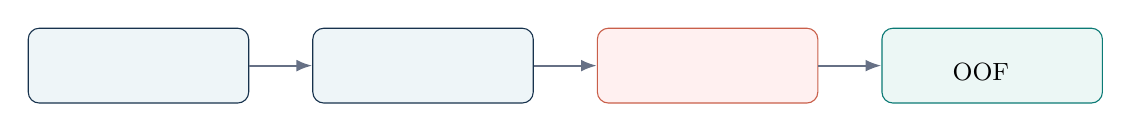
\begin{tikzpicture}[
  every node/.style={font=\small,align=center},
  train/.style={draw=DeepBlue,fill=SoftBlue,rounded corners=1.4mm,minimum width=2.8cm,minimum height=0.95cm},
  val/.style={draw=WarmGold,fill=SoftGold,rounded corners=1.4mm,minimum width=2.8cm,minimum height=0.95cm},
  test/.style={draw=Coral,fill=SoftRed,rounded corners=1.4mm,minimum width=2.8cm,minimum height=0.95cm},
  outputbox/.style={draw=PandaTeal,fill=SoftTeal,rounded corners=1.4mm,minimum width=2.8cm,minimum height=0.95cm},
  arrow/.style={-{Latex[length=2mm]},thick,color=MidGray}
]
\node[train] (inner) {外层训练集内部\\选择方法与超参数};
\node[train,right=8mm of inner] (refit) {完整外层训练集\\重拟合并冻结};
\node[test,right=8mm of refit] (test) {外层测试集\\只接收冻结变换};
\node[outputbox,right=8mm of test] (pred) {保存该折\\OOF 预测};
\draw[arrow] (inner)--(refit);
\draw[arrow] (refit)--(test);
\draw[arrow] (test)--(pred);
\end{tikzpicture}
\end{center}

五折测试预测拼接后，每个事件恰好出现一次：
\begin{equation}
  \widehat E_i^{\OOF}
  =\widehat E^{(-k(i))}(\symbf{x}_i),
  \qquad i=0,1,\ldots,4499.
\end{equation}

\begin{methodbox}[title={OOF 的准确含义},fonttitle=\bfseries]
生成事件 $i$ 的模型没有用事件 $i$ 训练或调参。OOF 宽度因此是留出事件上的样本外评价，而不是训练集拟合宽度，也不是挑选表现最好的一折。
\end{methodbox}

\begin{warningbox}[title={这一划分检验什么？},fonttitle=\bfseries]
它检验同一批数据中未参与训练事件的表现。它不构造时间外推，也不能单凭这一验证证明算法能迁移到另一个 run 或另一个采集时期。
\end{warningbox}
\clearpage

% -----------------------------------------------------------------------------
% 第 4 页：A0--A4
% -----------------------------------------------------------------------------
\section{逐通道物理矩阵：A0--A4}

第一条处理链先分别处理 $\SoneLY$ 与 $\StwoLY$，再用正权重组合为相对能量。五个候选在运行前固定，并使用完全相同的事件折。

\subsection*{3.1 固定候选}

\rowcolors{2}{SoftBlue}{white}
\begin{tabularx}{\textwidth}{@{}C{3.3cm} Y Y@{}}
\toprule
\rowcolor{DeepBlue!11}\textbf{候选} & \textbf{$\SoneLY$ 处理} & \textbf{$\StwoLY$ 处理}\\
\midrule
\texttt{A0\_raw} & 不做响应校正 & 不做响应校正\\
\texttt{A1\_s2\_lifetime} & 不校正 & 漂移时间指数趋势\\
\texttt{A2\_s1\_dt\_r2} & 先 $t_{\mathrm d}$，再 $r^2$ & 不校正\\
\texttt{A3\_s2\_lifetime\_r2} & 不校正 & 先指数趋势，再 $r^2$\\
\texttt{A4\_both} & 先 $t_{\mathrm d}$，再 $r^2$ & 先指数趋势，再 $r^2$\\
\bottomrule
\end{tabularx}

横向坐标只由读入的 $x,y$ 构造：
\begin{equation}
  r^2=x^2+y^2,
  \qquad
  t_{\mathrm d}=\frac{\texttt{dt}}{1000}\ [\mu\mathrm{s}].
\end{equation}

\subsection*{3.2 低自由度分箱响应}

对训练集中的信号 $q$ 和坐标 $z$，按 $z$ 的训练分位数划分 5 个近似等统计量箱。设第 $j$ 箱的稳健中心为 $c_j$，全训练集中心为 $c_0$，定义
\begin{equation}
  \rho_j=\frac{c_j}{c_0}.
\end{equation}
在箱中心之间线性插值 $\ln\rho_j$，得到 $\widehat{\ln\rho}(z)$；校正写为
\begin{equation}
  q^{\mathrm{corr}}
  =q\exp\!\left[-\widehat{\ln\rho}(z)\right].
\end{equation}
插值响应限制在 $[0.5,2.0]$ 内，避免稀疏边界产生数值爆炸。多个步骤按候选表中的顺序依次拟合，后一步只看前一步已经校正的训练信号。

\subsection*{3.3 S2 漂移时间趋势}

$\StwoLY$ 的指数步骤只拟合训练侧粗分箱中心：
\begin{equation}
  \ln c(t_{\mathrm d})
  =a+b\bigl(t_{\mathrm d}-t_0\bigr),
  \qquad
  -\frac{1}{200\,\mu\mathrm{s}}\le b\le0.
\end{equation}
非正斜率表达电子信号随漂移时间不增加的物理约束；这里得到的是当前样本中的表观趋势，不等同于正式电子寿命测量。

\subsection*{3.4 通道归一化与权重}

训练侧校正后中心记为 $c_1,c_2$，定义
\begin{equation}
  s_1=\frac{\SoneLY^{\mathrm{corr}}}{c_1},
  \qquad
  s_2=\frac{\StwoLY^{\mathrm{corr}}}{c_2},
\end{equation}
并在内层验证中选择
\begin{equation}
  e_{\alpha}=\alpha s_1+(1-\alpha)s_2,
  \qquad
  \alpha\in\{0.10,0.15,\ldots,0.90\}.
\end{equation}
先最小化内层 $\Rsixtyeight$，再以 $\Rninty$ 和较小的 $\alpha$ 依次打破平局。所有中心、响应与 $\alpha$ 随外层模型一起冻结。

\begin{boundarybox}[title={A0--A4 的统计身份},fonttitle=\bfseries]
每个候选都有完整 OOF 预测；但候选之间在当前 OOF 上进行比较仍属于开发阶段的探索。最终采用哪一条处理链，必须先冻结，再到真正独立的数据上验证。
\end{boundarybox}

% -----------------------------------------------------------------------------
% 第 5 页：basic 矩阵
% -----------------------------------------------------------------------------
\section{basic 响应矩阵与嵌套 winner}

第二条处理链先组合两个光信号，再对组合量学习低阶空间响应。它用于检验不同处理顺序，不与上一节共享权重定义，因此两条管线的 raw 数值只能各自做前后比较。

\subsection*{4.1 训练侧原始组合}

设外层训练集中的信号中位数为 $m_1,m_2$，则
\begin{equation}
  E_{\mathrm{raw}}
  =\frac{\StwoLY}{m_2}
  +\alpha\frac{\SoneLY}{m_1},
  \qquad \alpha>0.
\end{equation}
$\alpha$ 网格包含从 $0.05$ 到 $20$ 的 15 个对数等距点，并额外包含 $0.75,1.0,1.5$。每个方法都在外层训练集内部单独选择自己的 $\alpha$。

\subsection*{4.2 预先登记的方法族}

\footnotesize
\rowcolors{2}{SoftBlue}{white}
\begin{tabularx}{\textwidth}{@{}C{3.1cm} C{1.5cm} Y@{}}
\toprule
\rowcolor{DeepBlue!11}\textbf{方法} & \textbf{复杂度} & \textbf{处理顺序}\\
\midrule
\texttt{raw} & 0 & 只做正权重信号组合\\
\texttt{dt\_quad} & 3 & 一维 $t_{\mathrm d}$ 二次响应\\
\texttt{r2\_quad} & 3 & 一维 $r^2$ 二次响应\\
\texttt{dt\_r2\_joint} & 6 & $t_{\mathrm d}$ 与 $r^2$ 联合二次面\\
\texttt{dt\_then\_r2} & 6 & 先 $t_{\mathrm d}$，再 $r^2$\\
\texttt{r2\_then\_dt} & 6 & 先 $r^2$，再 $t_{\mathrm d}$\\
\texttt{xy\_quad} & 6 & $x,y$ 联合二次面\\
\texttt{dt\_then\_xy} & 9 & 先 $t_{\mathrm d}$，再 $x,y$\\
\texttt{dt\_r2\_then\_xy} & 12 & 联合 $t_{\mathrm d},r^2$ 后拟合 $x,y$ 残余\\
\bottomrule
\end{tabularx}
\normalsize

\subsection*{4.3 响应面拟合}

所有坐标先用训练中位数与训练尺度标准化。一维坐标划 10 个分位箱；二维坐标每维划 5 个分位箱。每个有效单元至少包含 12 个训练事件，拟合时只使用单元的坐标中位数、对数能量中位数与事件数。

一维和二维设计向量分别为
\begin{align}
  \symbf{\phi}_{1}(z)&=(1,z,z^2)^{\mathsf T},\\
  \symbf{\phi}_{2}(a,b)&=(1,a,b,a^2,b^2,ab)^{\mathsf T}.
\end{align}
以 $\sqrt{n_{\mathrm{cell}}}$ 加权并加入 $10^{-8}$ 的极小岭项求解 $\symbf{\beta}$。校正量为
\begin{equation}
  \Delta(\symbf z)
  =\symbf{\phi}(\symbf z)^{\mathsf T}\symbf{\beta}
  -\operatorname{median}_{\mathrm{train}}\!\left(\ln E\right),
  \qquad
  E^{\mathrm{corr}}=E\exp[-\Delta(\symbf z)].
\end{equation}
$\Delta$ 同时受训练预测的 1\%--99\% 范围和 $[-0.30,0.30]$ 限制。

\subsection*{4.4 嵌套 winner}

每个外层折中，九个方法先在训练侧分别选 $\alpha$。设内层最小宽度为 $R_{68}^{\star}$，将满足
\begin{equation}
  R_{68}^{(m)}\le R_{68}^{\star}+0.0005
\end{equation}
的方法视为近似并列，再优先选择复杂度最低者；若仍并列，再比较 $\Rsixtyeight$ 与 $\Rninty$。这个训练内选择结果称为 \texttt{nested\_winner}。

\begin{warningbox}[title={避免误解},fonttitle=\bfseries]
\texttt{nested\_winner} 不是在外层测试结果中挑最好方法。它在每个外层折的训练侧完成方法选择，然后只把已选模型应用到该折的 900 个测试事件。
\end{warningbox}

% -----------------------------------------------------------------------------
% 第 6 页：相对能量与指标
% -----------------------------------------------------------------------------
\section{相对能量、OOF 汇总与评价指标}

\subsection*{5.1 相对尺度}

任一外层模型都只用训练事件确定最终尺度 $s_E$，再对测试事件输出
\begin{equation}
  \widehat E_i^{\OOF}
  =\frac{e_i}{s_E}.
\end{equation}
因此 $\widehat E^{\OOF}$ 是中心约为 1 的无量纲相对量。五折拼接后，以全体 OOF 中位数
\begin{equation}
  Q_{50}=\operatorname{median}\!\left(\widehat E_0^{\OOF},\ldots,
  \widehat E_{4499}^{\OOF}\right)
\end{equation}
作为评价尺度，但这个全体中位数只用于计算最终指标，不反馈到任何外层模型。

\subsection*{5.2 主指标 $\Rsixtyeight$ 与 $\Rninty$}

令 $Q_p$ 表示全部有限 OOF 相对能量的第 $p$ 分位数，定义
\begin{align}
  \Rsixtyeight
  &=\frac{Q_{84.135}-Q_{15.865}}{2Q_{50}},\\
  \Rninty
  &=\frac{Q_{95}-Q_{5}}{2Q_{50}}.
\end{align}
$\Rsixtyeight$ 描述中心 68.27\% 事件的典型半宽，$\Rninty$ 描述更宽的中心 90\% 区域。二者均使用全部 4500 条 OOF 预测，不先选峰窗，也不删除尾部。

另外令
\begin{equation}
  y_i=\frac{\widehat E_i^{\OOF}}{Q_{50}},
\end{equation}
记录固定范围外事件比例和相对尾部比例：
\begin{align}
  f_{20}
  &=\frac{1}{N}\sum_{i=1}^{N}
  \mathbf 1\!\left(y_i<0.8\ \lor\ y_i>1.2\right),\\
  f_{2R}
  &=\frac{1}{N}\sum_{i=1}^{N}
  \mathbf 1\!\left(|y_i-1|>2\Rsixtyeight\right).
\end{align}

\begin{infobox}[title={为什么主报分位数宽度？},fonttitle=\bfseries]
当前能量分布可能包含非高斯尾部、上游预选边界和不均匀空间覆盖。分位数宽度不要求先指定峰形；同时报告 $\Rsixtyeight$、$\Rninty$ 与固定尾部比例，可以避免只看峰顶附近而忽略宽尾。
\end{infobox}

\subsection*{5.3 OOF 后的响应诊断}

为了检查剩余结构，可在所有 OOF 预测生成以后，分别按 $t_{\mathrm d}$ 与 $r^2$ 做等统计量分箱，计算每箱稳健中心相对于全局中心的变化。该诊断只描述留出事件中的残余趋势：
\begin{equation}
  \delta_j
  =\frac{c_j^{\OOF}}{c_{\mathrm{global}}^{\OOF}}-1.
\end{equation}
诊断结果不得反馈到当前响应图、权重或方法选择。

\begin{boundarybox}[title={这些量不是什么},fonttitle=\bfseries]
$\Rsixtyeight$ 与 $\Rninty$ 是当前预选样本的观测分布宽度，不是自动成立的高斯 $\sigma/\mu$，也不是已经完成绝对标定的探测器本征能量分辨率。
\end{boundarybox}

% -----------------------------------------------------------------------------
% 第 7 页：bootstrap 与输出
% -----------------------------------------------------------------------------
\section{配对事件 bootstrap 与结果追溯}

\subsection*{6.1 冻结 OOF 预测上的事件重采样}

在模型、超参数和全部 OOF 预测已经冻结后，进行 $B=1000$ 次事件级有放回抽样。第 $b$ 次复制从
\begin{equation}
  \{0,1,\ldots,N-1\}
\end{equation}
中独立抽取 $N=4500$ 个索引，得到
\begin{equation}
  \mathcal I_b=(i_{b1},i_{b2},\ldots,i_{bN}).
\end{equation}
同一组 $\mathcal I_b$ 同时用于 raw 与校正候选，因而比较保持配对。对宽度 $R\in\{\Rsixtyeight,\Rninty\}$，每次计算
\begin{align}
  \Delta R_b
  &=R_b^{\mathrm{corr}}-R_b^{\mathrm{raw}},\\
  \Gamma R_b
  &=\frac{R_b^{\mathrm{corr}}}{R_b^{\mathrm{raw}}}.
\end{align}
最终报告 $\Delta R_b$ 或 $\Gamma R_b$ 的 2.5\%、50\% 和 97.5\% 分位数。

\begin{methodbox}[title={“配对”的含义},fonttitle=\bfseries]
每次复制中，raw 与 corrected 使用完全相同的事件索引及重复次数。因此区间针对“同一批重采样事件上的前后差异”，不会把两次独立抽样的样本波动误算进方法差异。
\end{methodbox}

\begin{boundarybox}[title={bootstrap 的准确边界},fonttitle=\bfseries]
每次复制只重组已经生成的 OOF 预测，没有重新学习响应、重新选择权重或重新选择方法。因此该区间是\textbf{条件于冻结 OOF 预测的事件组成不确定度}，不是完整训练流水线的不确定度。
\end{boundarybox}

\subsection*{6.2 事件独立性假设}

事件级 bootstrap 把 4500 个事件视为可交换、近似独立的观测。如果实际存在未建模的时间相关、批次相关或共同探测器状态，区间可能偏窄。当前数据没有足够信息估计这类相关结构，因此报告必须保留这一限制，不能把“区间不跨零”解释成跨时期稳定。

\subsection*{6.3 输出与一一追溯}

\rowcolors{2}{SoftTeal}{white}
\begin{tabularx}{\textwidth}{@{}C{4.0cm} Y@{}}
\toprule
\rowcolor{PandaTeal!13}\textbf{输出类别} & \textbf{最少保留内容}\\
\midrule
逐事件 OOF 表 & \texttt{sourceRow}、外层折、候选或方法、训练侧选择结果、OOF 相对能量\\
逐折指标表 & 训练/测试事件数、内层选择、$\Rsixtyeight$、$\Rninty$ 与尾部指标\\
模型元数据 & 输入摘要、随机种子、折算法、候选定义、训练中心、响应参数与权重\\
事件 bootstrap 表 & 复制编号、raw/corrected 宽度、差值、比值与分位区间\\
\bottomrule
\end{tabularx}

\begin{infobox}[title={可复现性的最小条件},fonttitle=\bfseries]
必须同时保存输入内容指纹、原始行序、\texttt{sourceRow}、随机种子 10972、折生成算法和软件版本。仅保存一张最终直方图不足以重建训练/测试关系。
\end{infobox}
\clearpage

% -----------------------------------------------------------------------------
% 第 8 页：限制与结论
% -----------------------------------------------------------------------------
\section{方法边界、复现顺序与下一步}

\subsection*{7.1 建议复现顺序}

\begin{enumerate}
  \item 只读载入 7 个字段，按原始行序生成 \texttt{sourceRow}；
  \item 检查 4500 行的有限值、信号正值和 \texttt{sourceRow} 唯一性；
  \item 用种子 10972 生成平衡事件级五折，并保存折标签；
  \item 运行 A0--A4 通道矩阵，所有选择限制在外层训练侧；
  \item 运行 basic 方法矩阵及 \texttt{nested\_winner}；
  \item 拼接五折 OOF 预测，计算 $\Rsixtyeight$、$\Rninty$ 与尾部；
  \item 对冻结 OOF 预测执行 1000 次配对事件 bootstrap；
  \item 保存逐事件表、逐折表、模型参数、元数据和输入指纹。
\end{enumerate}

\subsection*{7.2 当前已经做到什么？}

\begin{methodbox}[title={已建立的处理链},fonttitle=\bfseries]
\begin{itemize}
  \item 只使用 5 个基本物理观测量建立独立重建，不借用已有能量分支；
  \item 对同一批 4500 个事件比较所有候选，没有通过额外删选人为缩窄分布；
  \item 用 \texttt{sourceRow} 保证输入、折标签与 OOF 结果一一对应；
  \item 将响应学习、归一化、权重与方法选择全部限制在训练侧；
  \item 同时保存逐事件 OOF、逐折指标、尾部诊断与配对事件重采样区间。
\end{itemize}
\end{methodbox}

\subsection*{7.3 当前不能声称什么？}

\begin{boundarybox}[title={必须保留的限制},fonttitle=\bfseries]
\begin{itemize}
  \item 只有 run10972，且上游 \texttt{Egt2MeV} 预选细节、源类型和目标单线尚未完全确认；
  \item 事件级五折只检验同一数据集内的留出事件，不能证明跨 run 或跨采集时期泛化；
  \item 事件 bootstrap 假定观测近似独立，未包含隐藏相关性和完整重训练不确定度；
  \item 当前输出是相对能量，尚未利用 $g_1$、$g_2$ 或已知峰能完成绝对标定；
  \item 当前样本空间覆盖不均匀，低阶响应可能同时吸收探测器响应与样本组成效应。
\end{itemize}
\end{boundarybox}

\subsection*{7.4 下一阶段的正确验证}

应先冻结候选定义、响应自由度、权重网格、折算法和评价指标，再取得未参与开发的独立校准 run。在新数据上不得重新挑选方案，只能应用冻结流程，并同时比较
\begin{equation}
  \Rsixtyeight,\qquad
  \Rninty,\qquad
  f_{20},\qquad
  \delta(t_{\mathrm d}),\qquad
  \delta(r^2).
\end{equation}

\begin{warningbox}[title={当前最严谨的总结},fonttitle=\bfseries]
本项目已经建立了“固定事件集合 $\rightarrow$ 确定性事件级嵌套 OOF $\rightarrow$ 训练内响应与方法选择 $\rightarrow$ 全事件非参数宽度 $\rightarrow$ 配对事件 bootstrap”的可追溯处理链。它可以评价 run10972 内留出事件的相对能量重建，但正式的跨 run 结论与绝对能量分辨率仍需独立数据验证。
\end{warningbox}

\end{document}
